\documentclass[10pt]{beamer}
\usepackage{uglixbeamer,animate}
\title{Arbres binaires de recherche}
\subtitle{Chapitre 14}
\author{NSI2}

\begin{document}

\maketitle

\begin{frame}{Définition}
Un arbre binaire de recherche est un arbre binaire\pause
\begin{enumerate}[--]
    \item dont tous les n\oe uds comportent des valeurs du même type qu'il est possible de comparer (entiers, flottants, chaînes de caractères...);\pause
    \item dont les valeurs de tous les n\oe uds situés dans le \alert{sous-arbre gauche} d'un n\oe ud sont \alert{inférieures ou égales} à la valeur de ce n\oe ud;\pause
\end{enumerate}
 
\end{frame}
\begin{frame}{Exemple}
Voici un ABR :
\begin{center}
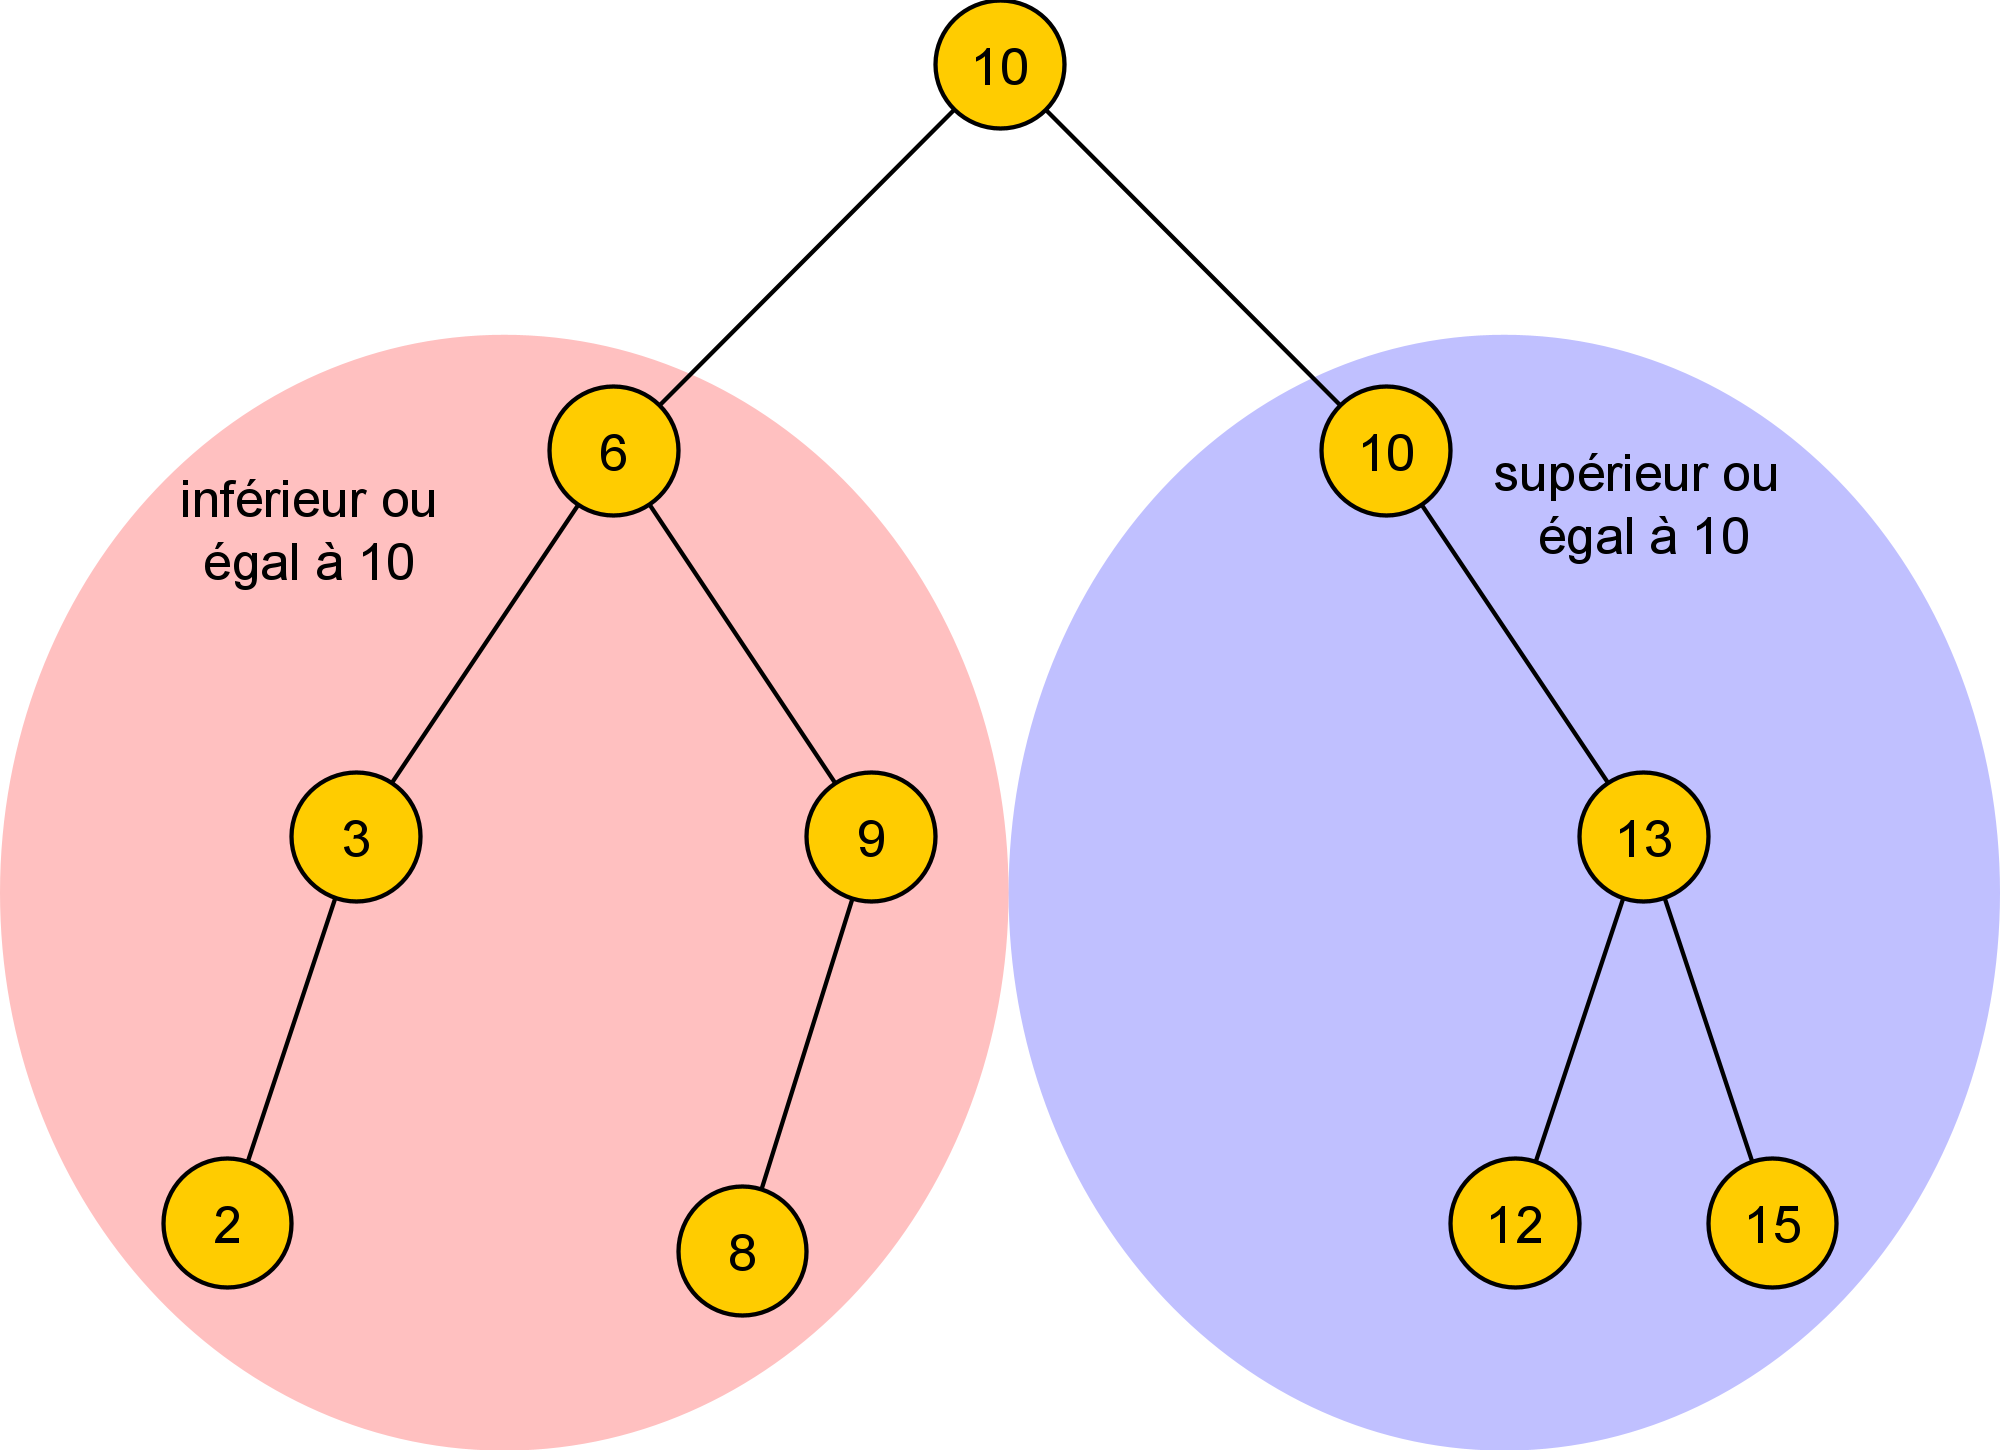
\includegraphics[width=7cm]{img/abr1}
\end{center}
\end{frame}
\begin{frame}{Exemple}
Ceci n'est pas un ABR
    \begin{center}
        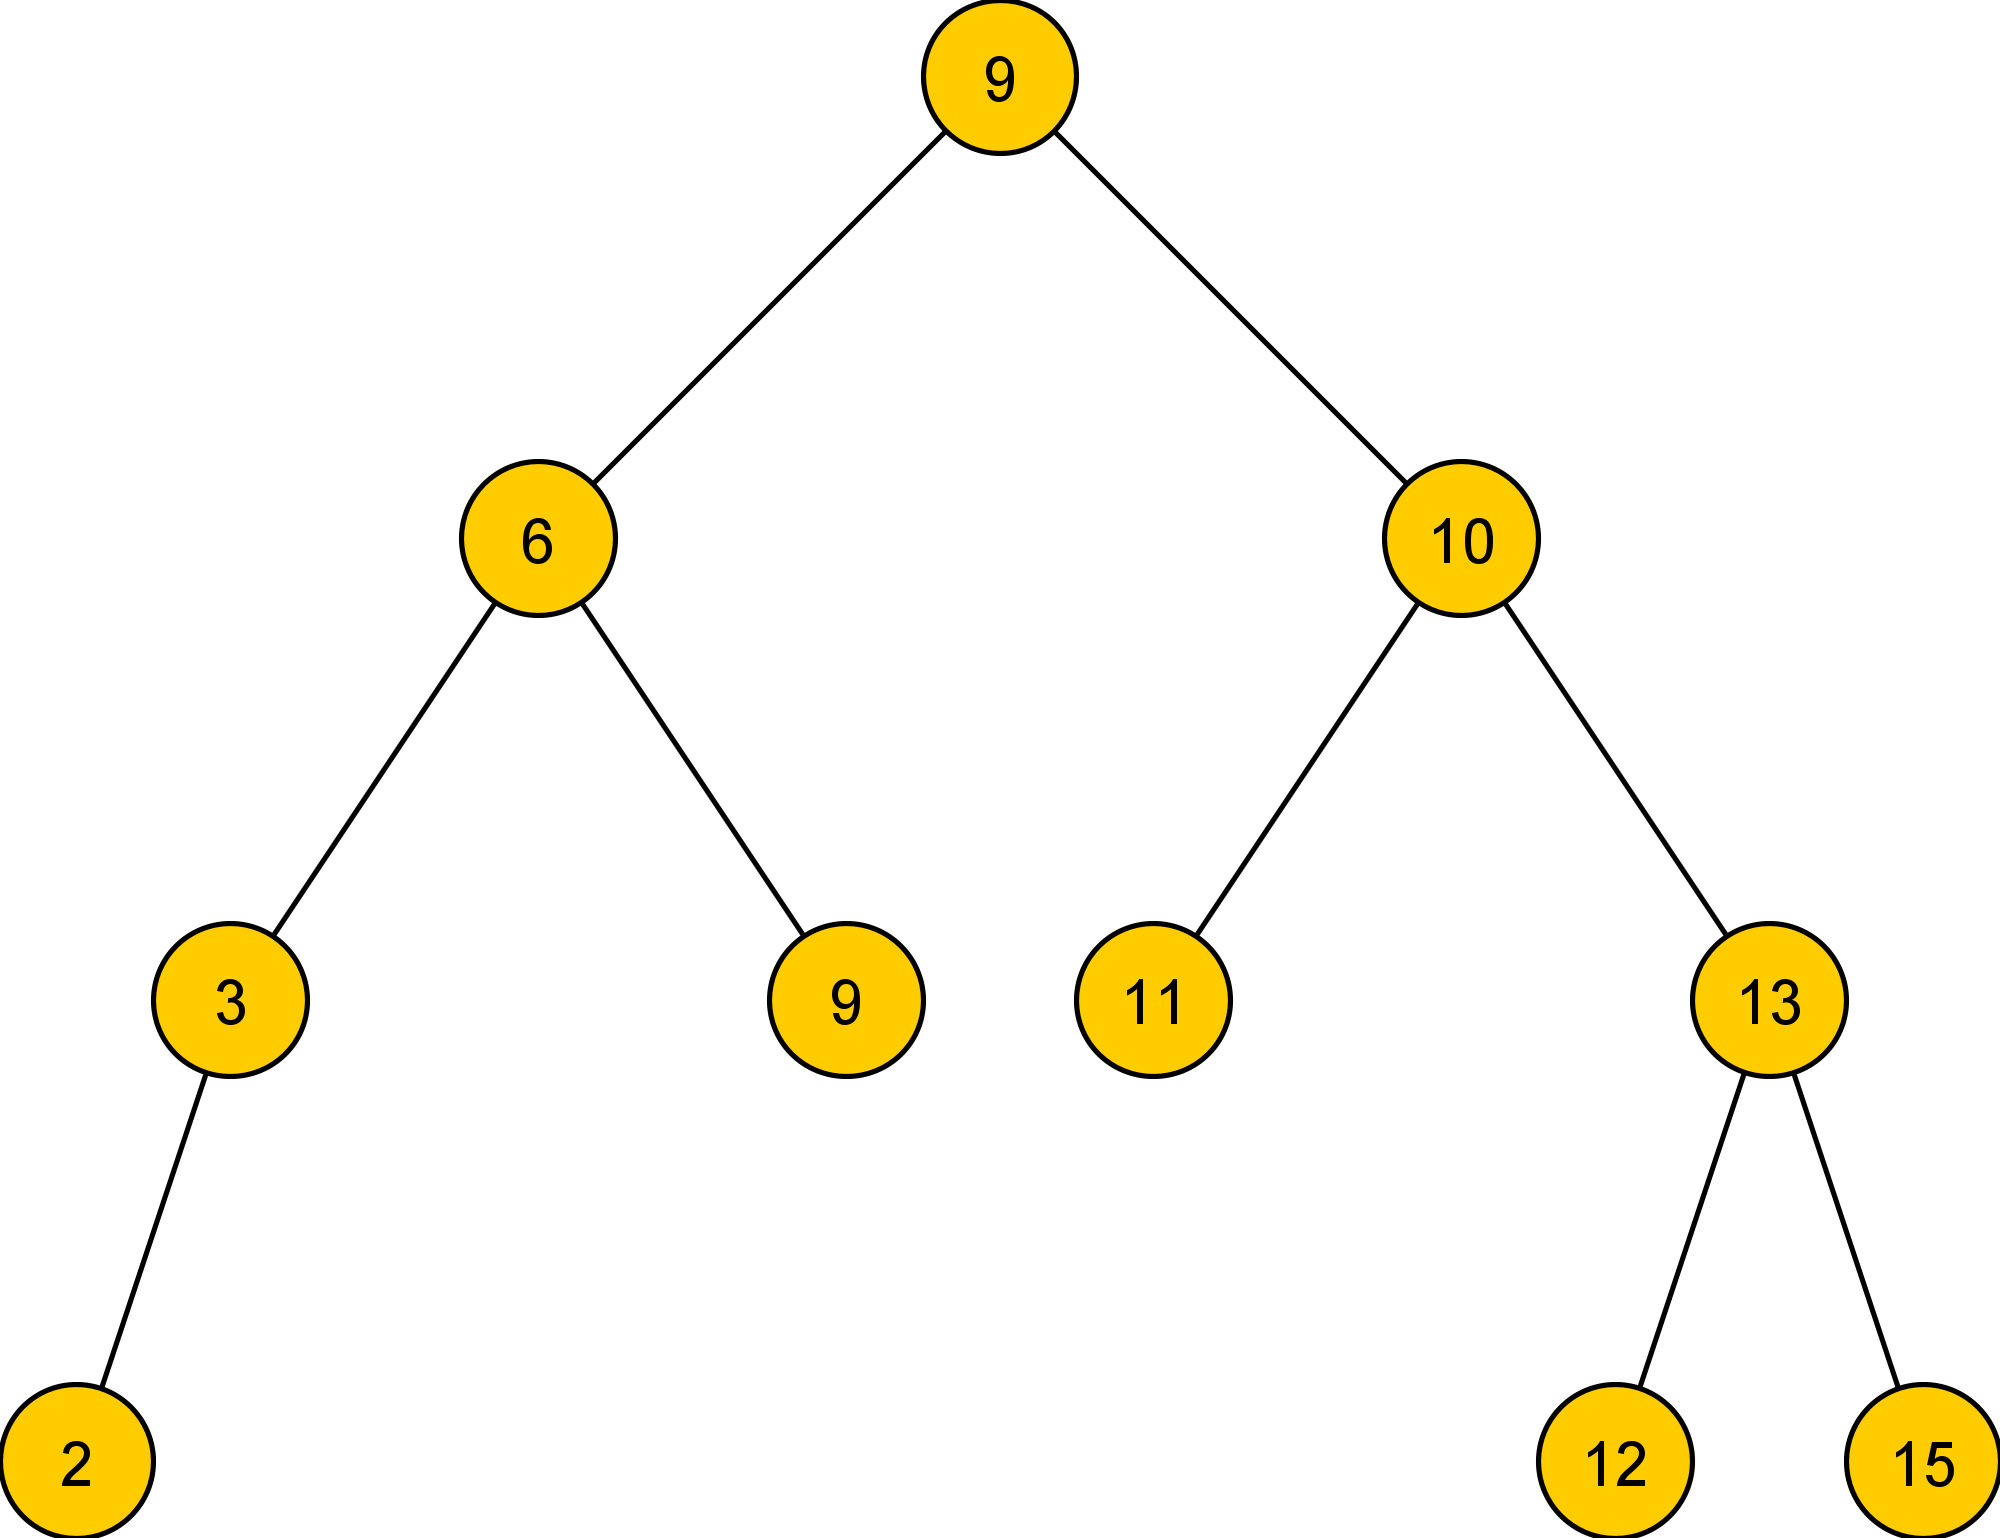
\includegraphics[width=7cm]{img/abr2}
    \end{center}
\end{frame}
\begin{frame}{Recherche dans un ABR}
        \begin{center}
        \animategraphics[step,width=7cm]{0.2}{img/recherche/recherche}{0}{4}
    \end{center}
\end{frame}
\begin{frame}{Recherche dans un ABR}
    \begin{center}
        \animategraphics[step,width=7cm]{0.2}{img/recherchebis/recherchebis}{0}{4}
    \end{center}
\end{frame}
\begin{frame}{Ajout d'un élément dans un ABR}
    \begin{center}
        \animategraphics[step,width=7cm]{0.2}{img/ajout/ajout}{0}{4}
    \end{center}
\end{frame}

\begin{frame}{Suppression d'un élément dans un ABR}
    \begin{center}
    \animategraphics[step,width=7cm]{0.2}{img/suppr/suppr}{0}{3}
    \end{center}

    \alert{Ceci est hors programme.}
\end{frame}
\section*{Intérêts}
\begin{frame}{Complexité}
Le coût de recherche ou d'ajout d'un élément dans un ABR est proportionnel à sa hauteur.\\

Dans le pire des cas, où l'ABR est dégénéré, on ne gagne pas grand chose par rapport à une liste.\\

Le meilleur des cas serait d'avoir un arbre parfait.\\
\end{frame}
\begin{frame}{\'Equilibrage}
Il existe des méthodes pour, lors de l'ajout  d'un élément dans un ABR, s'assurer que celui-ci reste bien \textit{équilibré}. Elles ne sont pas au programme de terminale.

Dans ce cas la hauteur $h$ de l'ABR est dite \textit{logarithmique}, c'est à dire que si $N$ désigne le nombre de n\oe uds, il existe une constante $C$ telle que $$h\leqslant C.\log_2(N)$$\\

Alors, avec un ABR équilibré, les opérations de recherche et d'ajouts sont très efficaces.
\end{frame}
\begin{frame}{Exemple}
Imaginons un ABR parfait de hauteur $h$, il possède $N=2^{h+1}-1$ éléments.\\
Le temps de recherche ou d'ajout d'un élément (dans le pire des cas) est proportionnel à $h$.\\

Prenons $h=50$, alors notre ABR comporte \np{2251799813685247} éléments, et on trouve ou on ajoute un nouvel élément en environ 50 étapes au maximum !
\end{frame}
\end{document}